\documentclass[]{beamer}
% Class options include: notes, notesonly, handout, trans,
%                        hidesubsections, shadesubsections,
%                        inrow, blue, red, grey, brown

% Theme for beamer presentation.
\usepackage{beamerthemesplit} 
% Other themes include: beamerthemebars, beamerthemelined, 
%                       beamerthemetree, beamerthemetreebars  

\title[Commitment Institutions and Instability]{Commitment Institutions and Electoral and Political Instability}
\subtitle{A Reduced-Form Approach}
\author{Isaac Liu}
\date{\today}

\usepackage{graphicx} % http://ctan.org/pkg/graphicx
\usepackage{amsmath}
\usepackage{geometry}
\usepackage{amsfonts}
\usepackage[english]{babel}
\usepackage{amssymb}
\usepackage{graphicx}
\usepackage{float}
\usepackage{hyperref}
\usepackage{multirow}
\usepackage{pdflscape}
\usepackage{caption}
\usepackage{pdflscape}
\usepackage{outlines}
\usepackage{subcaption}


\usepackage{tabularx, booktabs}

\usepackage{standalone}

\usepackage[autostyle, english = american]{csquotes}
\MakeOuterQuote{"}

\usepackage{comment}

\hypersetup{
    colorlinks=true,
    linkcolor=white,
    filecolor=black,      
    urlcolor=black,
}

\begin{document}

    \begin{frame}
        \titlepage
    \end{frame}

    \begin{frame}
        \frametitle{\small Do the commitment institutions of central bank independence and fixed exchange rates affect electoral and political instability?}
        \begin{itemize}
            \item Net Welfare Benefits
            \begin{itemize}
                \item Inflation Time Inconsistency
                \item Political efficacy, access to capital
                \item Economic Voting, Increased Stability
            \end{itemize}
            \item Political Business Cycles
            \begin{itemize}
                \item Inability to manipulate economy or satisfy partisans
                \item Monetary (perhaps fiscal) policy
                \item Economic voting, Decreased Stability
            \end{itemize}
        \end{itemize}

        \begin{figure}[h]
    
            \begin{subfigure}[h]{0.475\textwidth}
                \centering
                
\includegraphics[width=0.95\hsize]{../../Output/Figures/Fire_JP_Headline.png} 
            \end{subfigure}
            \hfill
            \begin{subfigure}[h]{0.475\textwidth}
                \centering
                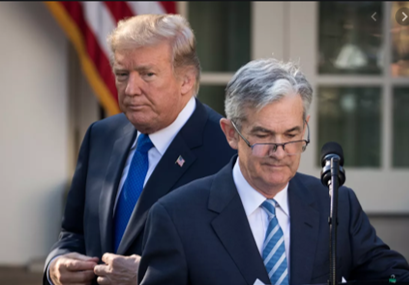
\includegraphics[width=0.95\hsize]{../../Output/Figures/Trump_and_JP.png}
            \end{subfigure}
    
        \end{figure}

    \end{frame}


    \begin{frame}
        \frametitle{Literature}
        \begin{itemize}
            \item Bernhard and Leblang (2002)
            \begin{itemize}
                \item OLS, 16 parliamentary democracies since 1970s
                \item CBI increases cabinet duration by 3mos, Fixed rates by 5mos
            \end{itemize}
            \item Clark, Golder, and Poast (2013)
            \begin{itemize}
                \item Survival Analysis, 19 OECD countries since 1970s
                \item Both institutions increase leader survival but only after 7y in office
            \end{itemize}
            \item Contribution:
            \begin{itemize}
                \item Far larger dataset including non/semi-democracies
                \item More consideration of endogeneity: choice of institutions based on stability consideration, de jure independence
                \item Political, not just electoral stability (coups, civil wars, etc), consideration for specific governmental positions
            \end{itemize}
        \end{itemize}
    \end{frame}


    \begin{frame}
        \frametitle{Data}
        \begin{itemize}
            \item Panel of 192 countries, 1970-2016
            \item Varieties of Democracy
            \begin{itemize}
                \item V2elturnhos, v2eltturnhog, v2eltvrig
                \item 0 for same individual, 1 for same party or coalition, 2 for new party \& ind.
                \item WGI Political Violence (neg = unstable)
                \item Instability Event- coup, civil war, internal conflict
            \end{itemize}
            \item Garriga (Cukierman, Webb, Neyapti)- de jure CBI
            \item Dreher et al.- Irregular turnover of governor- de facto CBI
            \item Reinhart, Rogoff Exchange Rates: 16 categories (higher = float)
        \end{itemize}
    \end{frame}


    \begin{frame}
        \frametitle{Results}
        \begin{itemize}
            \item FEs, clustered SEs
            \item De Jure CBI and more instability: PBCs
            \item Less De Facto CBI (high irregular turnover) and more lower chamber turnover
            \item Floating rate and HOS turnover
            \item Welfare Benefits of De Facto CBI, Fixed Rates?
        \end{itemize}
    \end{frame}

    \begin{frame}
        \frametitle{De Jure CBI and FIxed Rates}
        {
            \let\oldcentering\centering
            \renewcommand\centering{\tiny\oldcentering}
            {
\def\sym#1{\ifmmode^{#1}\else\(^{#1}\)\fi}
\begin{tabular}{l*{5}{c}}
\hline\hline
                &\multicolumn{1}{c}{(1)}&\multicolumn{1}{c}{(2)}&\multicolumn{1}{c}{(3)}&\multicolumn{1}{c}{(4)}&\multicolumn{1}{c}{(5)}\\
                &\multicolumn{1}{c}{Head of Govt. Turnover}&\multicolumn{1}{c}{Head of State Turnover}&\multicolumn{1}{c}{Lower House Turnover}&\multicolumn{1}{c}{WB Political Stability (Absence of Violence)}&\multicolumn{1}{c}{Instability Event Indicator}\\
\hline
De Jure CBI (CNW Index)&    0.276         &    0.303\sym{*}  &    0.389\sym{*}  &   -0.417\sym{**} &    1.000\sym{***}\\
                &   (1.44)         &   (2.30)         &   (1.99)         &  (-2.75)         &  (11.15)         \\
[1em]
Exchange Rate Classification (RR inverted, higher = more fixed)&  -0.0120         &  -0.0207\sym{***}& -0.00615         &   0.0106         &  0.00690         \\
                &  (-1.61)         &  (-3.45)         &  (-0.71)         &   (1.69)         &   (1.33)         \\
[1em]
Constant        &    0.618\sym{***}&    0.390\sym{***}&    0.535\sym{***}&   0.0283         &   -0.113\sym{*}  \\
                &   (6.15)         &   (5.43)         &   (4.99)         &   (0.31)         &  (-2.20)         \\
\hline
Observations    &     1399         &     1399         &     1141         &     2141         &     4207         \\
\hline\hline
\multicolumn{6}{l}{\footnotesize \textit{t} statistics in parentheses}\\
\multicolumn{6}{l}{\footnotesize \sym{*} \(p<0.05\), \sym{**} \(p<0.01\), \sym{***} \(p<0.001\)}\\
\end{tabular}
}

        }
    \end{frame}

    \begin{frame}
        \frametitle{De Facto CBI and FIxed Rates}
        {
            \let\oldcentering\centering
            \renewcommand\centering{\tiny\oldcentering}
            \begin{table}[htbp]\centering
\def\sym#1{\ifmmode^{#1}\else\(^{#1}\)\fi}
\caption{De Facto CBI, Fixed Effects Regression with Clustered Standard Errors \label{multIndFEDF}}
\begin{tabular}{l*{5}{c}}
\hline\hline
                    &\multicolumn{1}{c}{(1)}&\multicolumn{1}{c}{(2)}&\multicolumn{1}{c}{(3)}&\multicolumn{1}{c}{(4)}&\multicolumn{1}{c}{(5)}\\
                    &\multicolumn{1}{c}{Head of Govt. Turnover}&\multicolumn{1}{c}{Head of State Turnover}&\multicolumn{1}{c}{Lower House Turnover}&\multicolumn{1}{c}{WB Political Stability (Absence of Violence)}&\multicolumn{1}{c}{Instability Event Indicator}\\
\hline
(Lack of) Irregular &      -0.117         &     -0.0512         &      -0.211\sym{**} &     0.00955         &      0.0244         \\
CB Governor Turnover (higher = more de facto CBI)&     (-1.68)         &     (-0.81)         &     (-2.81)         &      (0.36)         &      (1.36)         \\
[1em]
Exchange Rate       &    -0.00548         &     -0.0117\sym{*}  &     0.00444         &      0.0153\sym{*}  &      0.0128\sym{**} \\
Classification (RR inverted, higher = more fixed)&     (-0.82)         &     (-2.06)         &      (0.53)         &      (2.08)         &      (2.73)         \\
[1em]
Constant            &       0.805\sym{***}&       0.521\sym{***}&       0.865\sym{***}&      -0.247\sym{***}&       0.261\sym{***}\\
                    &      (9.91)         &      (7.75)         &      (9.43)         &     (-3.54)         &      (6.77)         \\
\hline
Observations        &        1651         &        1651         &        1334         &        2669         &        4491         \\
\hline\hline
\multicolumn{6}{l}{\footnotesize \textit{t} statistics in parentheses}\\
\multicolumn{6}{l}{\footnotesize \sym{*} \(p<0.05\), \sym{**} \(p<0.01\), \sym{***} \(p<0.001\)}\\
\end{tabular}
\end{table}

        }
    \end{frame}

    \begin{frame}
        \frametitle{Ordered Logit (Mean Marginal Effects)}
        \begin{itemize}
            \item Nothing changes in terms of significance, except for fixed Erates and HOG
            \item xtologit; random effects
        \end{itemize}
        {
\def\sym#1{\ifmmode^{#1}\else\(^{#1}\)\fi}
\begin{tabular*}{\linewidth}{@{\hskip\tabcolsep\extracolsep\fill}l*{3}{c}}
\hline\hline
                &\multicolumn{1}{c}{(1)}&\multicolumn{1}{c}{(2)}&\multicolumn{1}{c}{(3)}\\
                &\multicolumn{1}{c}{}&\multicolumn{1}{c}{}&\multicolumn{1}{c}{}\\
\hline
De Jure CBI (CNW Index)&                  &                  &                  \\
1.\_predict      &   -0.146         &   -0.208\sym{***}&   -0.316\sym{***}\\
                &  (-1.93)         &  (-3.54)         &  (-3.65)         \\
[1em]
2.\_predict      &   0.0152         &   0.0390\sym{***}&   0.0980\sym{**} \\
                &   (1.80)         &   (3.32)         &   (3.21)         \\
[1em]
3.\_predict      &    0.131         &    0.169\sym{***}&    0.218\sym{***}\\
                &   (1.93)         &   (3.47)         &   (3.68)         \\
\hline
Exchange Rate Classification (RR inverted, higher = more fixed)&                  &                  &                  \\
1.\_predict      &  0.00792\sym{*}  &  0.00896\sym{**} &  0.00392         \\
                &   (2.45)         &   (3.21)         &   (0.96)         \\
[1em]
2.\_predict      &-0.000826\sym{*}  & -0.00168\sym{**} & -0.00122         \\
                &  (-2.22)         &  (-3.00)         &  (-0.96)         \\
[1em]
3.\_predict      & -0.00710\sym{*}  & -0.00728\sym{**} & -0.00271         \\
                &  (-2.46)         &  (-3.18)         &  (-0.96)         \\
\hline
Observations    &     1399         &     1399         &     1141         \\
\hline\hline
\multicolumn{4}{l}{\footnotesize \textit{t} statistics in parentheses}\\
\multicolumn{4}{l}{\footnotesize \sym{*} \(p<0.05\), \sym{**} \(p<0.01\), \sym{***} \(p<0.001\)}\\
\end{tabular*}
}

        \begin{table}[htbp]\centering
\def\sym#1{\ifmmode^{#1}\else\(^{#1}\)\fi}
\caption{De Facto CBI, Mean Marginal Effects, Ordered Logit Panel Regression, Random Effects, Clustered Standard Errors \label{ordLogDF}}
\begin{tabular}{l*{3}{c}}
\toprule
                                        &\multicolumn{1}{c}{(1)}&\multicolumn{1}{c}{(2)}&\multicolumn{1}{c}{(3)}\\
                                        &\multicolumn{1}{c}{}&\multicolumn{1}{c}{}&\multicolumn{1}{c}{}\\
\midrule
(Lack of) Irregular CB Governor Turnover (higher = more de facto CBI)&                  &                  &                  \\
1.\_predict                              &   0.0734\sym{*}  &   0.0356         &    0.119\sym{**} \\
                                        &   (2.23)         &   (1.30)         &   (3.19)         \\
\addlinespace
2.\_predict                              & -0.00756\sym{*}  & -0.00655         &  -0.0296\sym{**} \\
                                        &  (-2.02)         &  (-1.24)         &  (-3.05)         \\
\addlinespace
3.\_predict                              &  -0.0658\sym{*}  &  -0.0290         &  -0.0890\sym{**} \\
                                        &  (-2.23)         &  (-1.31)         &  (-3.14)         \\
\midrule
Exchange Rate Classification (RR inverted, higher = more fixed)&                  &                  &                  \\
1.\_predict                              &  0.00384         &  0.00473         & -0.00440         \\
                                        &   (1.32)         &   (1.93)         &  (-1.19)         \\
\addlinespace
2.\_predict                              &-0.000396         &-0.000870         &  0.00110         \\
                                        &  (-1.27)         &  (-1.87)         &   (1.18)         \\
\addlinespace
3.\_predict                              & -0.00345         & -0.00386         &  0.00331         \\
                                        &  (-1.32)         &  (-1.92)         &   (1.19)         \\
\midrule
Observations                            &     1651         &     1651         &     1334         \\
\bottomrule
\multicolumn{4}{l}{\footnotesize \textit{t} statistics in parentheses}\\
\multicolumn{4}{l}{\footnotesize \sym{*} \(p<0.05\), \sym{**} \(p<0.01\), \sym{***} \(p<0.001\)}\\
\end{tabular}
\end{table}

    \end{frame}


    \begin{frame}
        \frametitle{Panel Logit (binary instability event variable) Mean Marginal Effects}
        \begin{itemize}
            \item Fixed effects
            \item More evidence that de jure CBI increases political instability
            \item Fixed exchange rate (low RR rate) increases pol. instability, but very small effect size
        \end{itemize}
        \begin{table}[htbp]\centering
\def\sym#1{\ifmmode^{#1}\else\(^{#1}\)\fi}
\caption{De Jure CBI, Instability Event Panel Logit, Fixed Effects and Clustered Standard Errors, Mean Marginal Effects \label{margsJustBinInstabEventDJ}}
\begin{tabular}{l*{1}{c}}
\toprule
                                        &\multicolumn{1}{c}{(1)}\\
                                        &\multicolumn{1}{c}{}\\
\midrule
De Jure CBI (CNW Index)                 &     0.376\sym{***}\\
                                        &   (12.93)         \\
\addlinespace
Exchange Rate Classification (RR        &   0.00227\sym{**} \\
inverted, higher = more fixed)          &    (2.99)         \\
\midrule
Observations                            &      3912         \\
\bottomrule
\multicolumn{2}{l}{\footnotesize \textit{t} statistics in parentheses}\\
\multicolumn{2}{l}{\footnotesize \sym{*} \(p<0.05\), \sym{**} \(p<0.01\), \sym{***} \(p<0.001\)}\\
\end{tabular}
\end{table}

        \begin{table}[htbp]\centering
\def\sym#1{\ifmmode^{#1}\else\(^{#1}\)\fi}
\caption{Instability Event Panel Logit, Fixed Effects and Clustered Standard Errors, Mean Marginal Effects \label{margsJustBinInstabEventDF}}
\begin{tabular}{l*{1}{c}}
\toprule
                                        &\multicolumn{1}{c}{(1)}\\
                                        &\multicolumn{1}{c}{}\\
\midrule
De facto CBI                            &   0.0282         \\
                                        &   (1.18)         \\
\addlinespace
Fixed Rate                              &   0.0152\sym{***}\\
                                        &   (6.71)         \\
\midrule
Observations                            &     4163         \\
\bottomrule
\multicolumn{2}{l}{\footnotesize \textit{t} statistics in parentheses}\\
\multicolumn{2}{l}{\footnotesize \sym{*} \(p<0.05\), \sym{**} \(p<0.01\), \sym{***} \(p<0.001\)}\\
\end{tabular}
\end{table}

    \end{frame}


    \begin{frame}
        \frametitle{IV1: Tertiary Ed Enrollment (CBI), Aggregate GDP (Fixed Rate)}
        \begin{itemize}
            \item Good first stages
            \item Poor exclusion restrictions for political stability, better ones for electoral stability/turnover
            \item De jure CBI now increases lower chamber turnover, but no longer HOS
            \item Unclear sign for fixed rates (last two cols)
            \item De facto CBI omitted, insignificant
        \end{itemize}
        {
\def\sym#1{\ifmmode^{#1}\else\(^{#1}\)\fi}
\begin{tabular*}{\linewidth}{@{\hskip\tabcolsep\extracolsep\fill}l*{5}{c}}
\toprule
                &\multicolumn{1}{c}{(1)}&\multicolumn{1}{c}{(2)}&\multicolumn{1}{c}{(3)}&\multicolumn{1}{c}{(4)}&\multicolumn{1}{c}{(5)}\\
                &\multicolumn{1}{c}{Head of Govt. Turnover}&\multicolumn{1}{c}{Head of State Turnover}&\multicolumn{1}{c}{Lower House Turnover}&\multicolumn{1}{c}{WB Political Stability (Absence of Violence)}&\multicolumn{1}{c}{Instability Event Indicator}\\
\midrule
De Jure CBI (CNW Index)&    0.629         &   -0.478         &    0.847\sym{*}  &    6.976\sym{***}&    0.835\sym{***}\\
                &   (1.55)         &  (-1.42)         &   (1.97)         &  (13.27)         &   (4.30)         \\
\addlinespace
Exchange Rate Classification (RR inverted, higher = more fixed)& -0.00669         &   0.0171         &   0.0266         &  -0.0865\sym{**} &  -0.0295         \\
                &  (-0.19)         &   (0.51)         &   (0.76)         &  (-2.84)         &  (-1.66)         \\
\addlinespace
Constant        &    0.401         &    0.576\sym{*}  &   0.0636         &   -3.422\sym{***}&    0.292         \\
                &   (1.28)         &   (2.01)         &   (0.22)         &  (-9.22)         &   (1.65)         \\
\midrule
Observations    &      851         &      851         &      686         &     1865         &     2047         \\
\bottomrule
\multicolumn{6}{l}{\footnotesize \textit{t} statistics in parentheses}\\
\multicolumn{6}{l}{\footnotesize \sym{*} \(p<0.05\), \sym{**} \(p<0.01\), \sym{***} \(p<0.001\)}\\
\end{tabular*}
}

        {
\def\sym#1{\ifmmode^{#1}\else\(^{#1}\)\fi}
\begin{tabular}{l*{5}{c}}
\hline\hline
                    &\multicolumn{1}{c}{(1)}&\multicolumn{1}{c}{(2)}&\multicolumn{1}{c}{(3)}&\multicolumn{1}{c}{(4)}&\multicolumn{1}{c}{(5)}\\
                    &\multicolumn{1}{c}{Head of Govt. Turnover}&\multicolumn{1}{c}{Head of State Turnover}&\multicolumn{1}{c}{Lower House Turnover}&\multicolumn{1}{c}{WB Political Stability (Absence of Violence)}&\multicolumn{1}{c}{Instability Event Indicator}\\
\hline
(Lack of) Irregular &       1.295         &      -0.626         &       2.071         &       39.47\sym{*}  &      -18.01         \\
CB Governor Turnover (higher = more de facto CBI)&      (1.19)         &     (-0.74)         &      (1.66)         &      (1.97)         &     (-0.46)         \\
[1em]
Exchange Rate       &      0.0152         &     -0.0101         &      0.0864\sym{*}  &       0.581         &      -0.131         \\
Classification (RR inverted, higher = more fixed)&      (0.46)         &     (-0.32)         &      (2.08)         &      (1.49)         &     (-0.47)         \\
[1em]
Constant            &      -0.538         &       1.085         &      -1.708         &      -40.72         &       17.29         \\
                    &     (-0.50)         &      (1.32)         &     (-1.39)         &     (-1.96)         &      (0.48)         \\
\hline
Observations        &         962         &         962         &         788         &        2236         &        2011         \\
\hline\hline
\multicolumn{6}{l}{\footnotesize \textit{t} statistics in parentheses}\\
\multicolumn{6}{l}{\footnotesize \sym{*} \(p<0.05\), \sym{**} \(p<0.01\), \sym{***} \(p<0.001\)}\\
\end{tabular}
}

    \end{frame}


    \begin{frame}
        \frametitle{IV2: Population Share Social Science/Business Grads (CBI), Agg GDP (Fixed Rates)}
        \begin{itemize}
            \item Better Exclusion Restriction
            \item Very limited data but strong result for de jure CBI and political instability
        \end{itemize}
        \begin{table}[htbp]\centering
\def\sym#1{\ifmmode^{#1}\else\(^{#1}\)\fi}
\caption{Instruments of Social Science/Business Graduates Population Share and Aggregate GDP, Robust Standard Errors \label{ifivs3}}
\begin{tabular}{l*{5}{c}}
\toprule
                                        &\multicolumn{1}{c}{(1)}&\multicolumn{1}{c}{(2)}&\multicolumn{1}{c}{(3)}&\multicolumn{1}{c}{(4)}&\multicolumn{1}{c}{(5)}\\
                                        &\multicolumn{1}{c}{HoG Turnover}&\multicolumn{1}{c}{HoS Turnover}&\multicolumn{1}{c}{L. H. Turnover}&\multicolumn{1}{c}{WB Pol. Stability}&\multicolumn{1}{c}{Instab. Event}\\
\midrule
De Jure CBI                             &    44.33         &    14.48         &   -22.04         &   -19.44         &    2.704\sym{***}\\
                                        &   (0.49)         &   (0.47)         &  (-0.48)         &  (-0.24)         &   (4.11)         \\
\addlinespace
Fixed Rate                              &   -1.277         &   -0.422         &    0.704         &    0.722         &   -0.129         \\
                                        &  (-0.47)         &  (-0.44)         &   (0.51)         &   (0.27)         &  (-1.60)         \\
\addlinespace
Constant                                &   -19.38         &   -6.144         &    10.39         &    8.414         &                  \\
                                        &  (-0.50)         &  (-0.46)         &   (0.52)         &   (0.25)         &                  \\
\midrule
Observations                            &       20         &       20         &       17         &       53         &       12         \\
\bottomrule
\multicolumn{6}{l}{\footnotesize \textit{t} statistics in parentheses}\\
\multicolumn{6}{l}{\footnotesize \sym{*} \(p<0.05\), \sym{**} \(p<0.01\), \sym{***} \(p<0.001\)}\\
\end{tabular}
\end{table}

        {
\def\sym#1{\ifmmode^{#1}\else\(^{#1}\)\fi}
\begin{tabular}{l*{4}{c}}
\hline\hline
                    &\multicolumn{1}{c}{(1)}&\multicolumn{1}{c}{(2)}&\multicolumn{1}{c}{(3)}&\multicolumn{1}{c}{(4)}\\
                    &\multicolumn{1}{c}{Head of Govt. Turnover}&\multicolumn{1}{c}{Head of State Turnover}&\multicolumn{1}{c}{Lower House Turnover}&\multicolumn{1}{c}{WB Political Stability (Absence of Violence)}\\
\hline
(Lack of) Irregular &      -18.95         &      -5.278         &       19.37         &      -7.488         \\
CB Governor Turnover (higher = more de facto CBI)&     (-0.83)         &     (-0.40)         &      (0.80)         &     (-0.66)         \\
[1em]
Exchange Rate       &      0.0129         &     -0.0133         &       0.131\sym{*}  &      0.0659         \\
Classification (RR inverted, higher = more fixed)&      (0.22)         &     (-0.25)         &      (2.07)         &      (1.16)         \\
[1em]
Constant            &       19.38         &       5.799         &      -19.06         &       7.212         \\
                    &      (0.85)         &      (0.44)         &     (-0.79)         &      (0.64)         \\
\hline
Observations        &          59         &          59         &          52         &         187         \\
\hline\hline
\multicolumn{5}{l}{\footnotesize \textit{t} statistics in parentheses}\\
\multicolumn{5}{l}{\footnotesize \sym{*} \(p<0.05\), \sym{**} \(p<0.01\), \sym{***} \(p<0.001\)}\\
\end{tabular}
}

    \end{frame}


    \begin{frame}
        \frametitle{Just Aggregate GDP for Fixed Rates}
        \begin{itemize}
            \item Clearer case for fixed rates decreasing pol and electoral stability (PBC)
            \item Note on exclusion restriction: still an imperfect case
            \begin{itemize}
                \item Agg GDP proxies for economy size (optimum currency area)
                \item Arguably not as connected to GDP per capita to stability
            \end{itemize}
            \item Result for LH sensitive to dataset
        \end{itemize}
        \begin{table}[htbp]\centering
\def\sym#1{\ifmmode^{#1}\else\(^{#1}\)\fi}
\caption{Instrument of Aggregate GDP for Fixed Exchange Rates, Robust Standard Errors \label{miniRRIVs}}
\begin{tabular}{l*{2}{c}}
\toprule
                                        &\multicolumn{1}{c}{(1)}&\multicolumn{1}{c}{(2)}\\
                                        &\multicolumn{1}{c}{L. H. Turnover}&\multicolumn{1}{c}{WB Pol. Stability}\\
\midrule
Fixed Rate                              &   0.0779\sym{***}&   -0.257\sym{***}\\
                                        &   (3.35)         &  (-4.13)         \\
\addlinespace
Constant                                &   0.0991         &    1.992\sym{***}\\
                                        &   (0.58)         &   (4.16)         \\
\midrule
Observations                            &      835         &      437         \\
\bottomrule
\multicolumn{3}{l}{\footnotesize \textit{t} statistics in parentheses}\\
\multicolumn{3}{l}{\footnotesize \sym{*} \(p<0.05\), \sym{**} \(p<0.01\), \sym{***} \(p<0.001\)}\\
\end{tabular}
\end{table}

    \end{frame}


    \begin{frame}
        \frametitle{Table of Lags (see paper)}
        \begin{itemize}
            \item Irregular central bank turnover instantaneously associated with lower chamber election turnover
            \item T-3 sees strongest de jure CBI political instability impact
            \item T-6, T-8 de jure CBI increases pol instability. T-8 reduces HOG turnover (electoral instability) (similar to Clark, Golder, and Poast).
            \item Fixed rates increase instability in the same T-6 and up range
            \item Little significance for de facto CBI/governor turnover
        \end{itemize}
    \end{frame}


    \begin{frame}
        \frametitle{Summary}
        \begin{itemize}
            \item De jure CBI generally decreases (esp. pol) stability, suggesting limits on PBCs
            \item Sign unclear for governor turnover/de facto CBI
            \item Fixed exchange rates also increase electoral stability, but decrease political stability in FE \& XTLogit models
            \item In IV and lag specifications fixed rates decrease all stability
            \item Commitment institutions politically costly, at odds with literature
            \item Robust results
            \begin{itemize}
                \item Not covered: capital controls/openness don’t matter, binary independent variables somewhat reduce effect sizes, interactions with democracy do not matter, institutional controls for federalism and corporatism do not affect signs or cause large changes in effects
            \end{itemize}
        \end{itemize}
    \end{frame}


    \begin{frame}
        \frametitle{Questions/future directions}
        \begin{itemize}
            \item Diverging predictions for Head of Government, Head of State, Lower House Turnover
            \begin{itemize}
                \item HOS and Lower House seem to have strongest relationships
            \end{itemize}
            \item Endogenous elections
            \item Dynamic panel (A-Bond)?
            \item Ordinal logit regression with IV (different procedure)
        \end{itemize}
    \end{frame}


    \begin{frame}
        \centering Additional Results/Checks
    \end{frame}


    \begin{frame}
        \frametitle{Controls}
        \begin{itemize}
            \item Regional government exists and has autonomy and authority, checks and balances/horizontal accountability
            \item Not strictly necessary
        \begin{itemize}
            \item FEs
            \item No sign flips
        \end{itemize}
            \item Omitted: Corporatism
            \item Collinearity?
        \end{itemize}
        %\input{img0012.png}
    \end{frame}


    \begin{frame}
        \frametitle{HOS = HOG?}
        \begin{itemize}
            \item V2exhoshog is an indicator for whether HOS and HOG are the same person
            \item De jure CBI increases HOS turnover somewhat more when they are not the same person ???
            \item Weaker effect when they are
            \item Fixed erates reduce turnover in when they are the same person
        \end{itemize}
        %\input{img0009.png}
    \end{frame}


    \begin{frame}
        \frametitle{Democracy/Nondemocracy}
        \begin{itemize}
            \item High polity on the left, low polity on the right
            \item De facto CBI (less irregular turnover) means less lower chamber turnover in democracies but reverse in autocracies. Rule of law?
        \end{itemize}
        %\input{img0013.png}
        %\input{img0014.png}
    \end{frame}

\end{document}
